\selectlanguage{italian}%

\section{Soluzione}


\subsection{Schematici}

\begin{figure}[H]
	\centering
	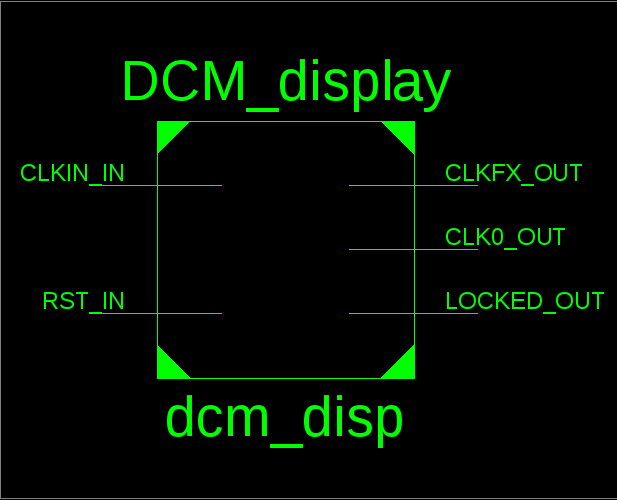
\includegraphics[scale=0.6]{esercizio05/images/DCM_display.png}
	\caption{Architettura del display a sette segmenti}
	\label{fig:display}
\end{figure}

Utilizzando il wizard di xilinx per la creazione degli ip core, possiamo
chiedere di creare un DCM che con un a frequenza in input di 50 MHz
ci restituisca in uscita un segnale periodico con frequenza di 5 MHz,
la frequenza desiderata � molto alta rispetto a quella che basterebbe
per visualizzare le cifre sul display, infatti si notano alcuni sfarfalii,
si potrebbe risolvere utilizzando una struttura a doppio DCM, per
far si che il numero di possibili frequenze a disposizioni aumentino,
ci accontentiamo della soluzione ad un singolo DCM essendo le cifre
visibili sul display.

\subsection{Codice}

Fare riferimento al codice del display \ref{fig:display}.

\selectlanguage{italian}%

